\documentclass[11pt]{article}
\usepackage[utf8]{inputenc}
\usepackage[T1]{fontenc}
\usepackage{graphicx}
\usepackage{longtable}
\usepackage{float}
\usepackage{wrapfig}
\usepackage{soul}
\usepackage{amssymb}
\usepackage{hyperref}
\usepackage[spanish]{babel}
\usepackage{bookman}
\usepackage[left=3cm,top=3cm,right=2cm,bottom=1cm,head=1.5cm,includefoot]{geometry}
\usepackage{listings}
\usepackage{multirow}
\usepackage{amssymb}
\usepackage{fancyhdr}
\usepackage{comment}
\usepackage{color}
\usepackage{multicol}
\usepackage[table]{xcolor}
\usepackage{ulem}

\title{informe}
\author{}

\begin{document}


\definecolor{gray97}{gray}{.97}
\definecolor{gray75}{gray}{.75}
\definecolor{gray45}{gray}{.45}

\lstset{linewidth=\textwidth}
\lstset{ frame=Ltb,
     framerule=0pt,
     aboveskip=0.5cm,
     framextopmargin=3pt,
     framexbottommargin=3pt,
     framexleftmargin=0.4cm,
     framesep=0pt,
     rulesep=.4pt,
     backgroundcolor=\color{gray97},
     rulesepcolor=\color{black},
     %
     stringstyle=\ttfamily,
     showstringspaces = false,
     basicstyle=\small\ttfamily,
     commentstyle=\color{gray45},
     keywordstyle=\bfseries,
     %
     numbers=left,
     numbersep=15pt,
     numberstyle=\tiny,
     numberfirstline = false,
     breaklines=true,
}


\pagestyle{fancy}
\lhead{
\includegraphics[width=1.5cm]{Logo-fiuba} }
\chead{75.59 - T\'ecnicas de Programaci\'on Concurrente I}
\rhead{\Huge FIUBA}
\lfoot{Trabajo Pr\'actico 2 }
\rfoot{$2^{do}$ cuatrimestre 2011}
\tableofcontents
\newpage


\section{Enunciado}

\begin{center}
% Orden del trim = izq abajo derecha arriba
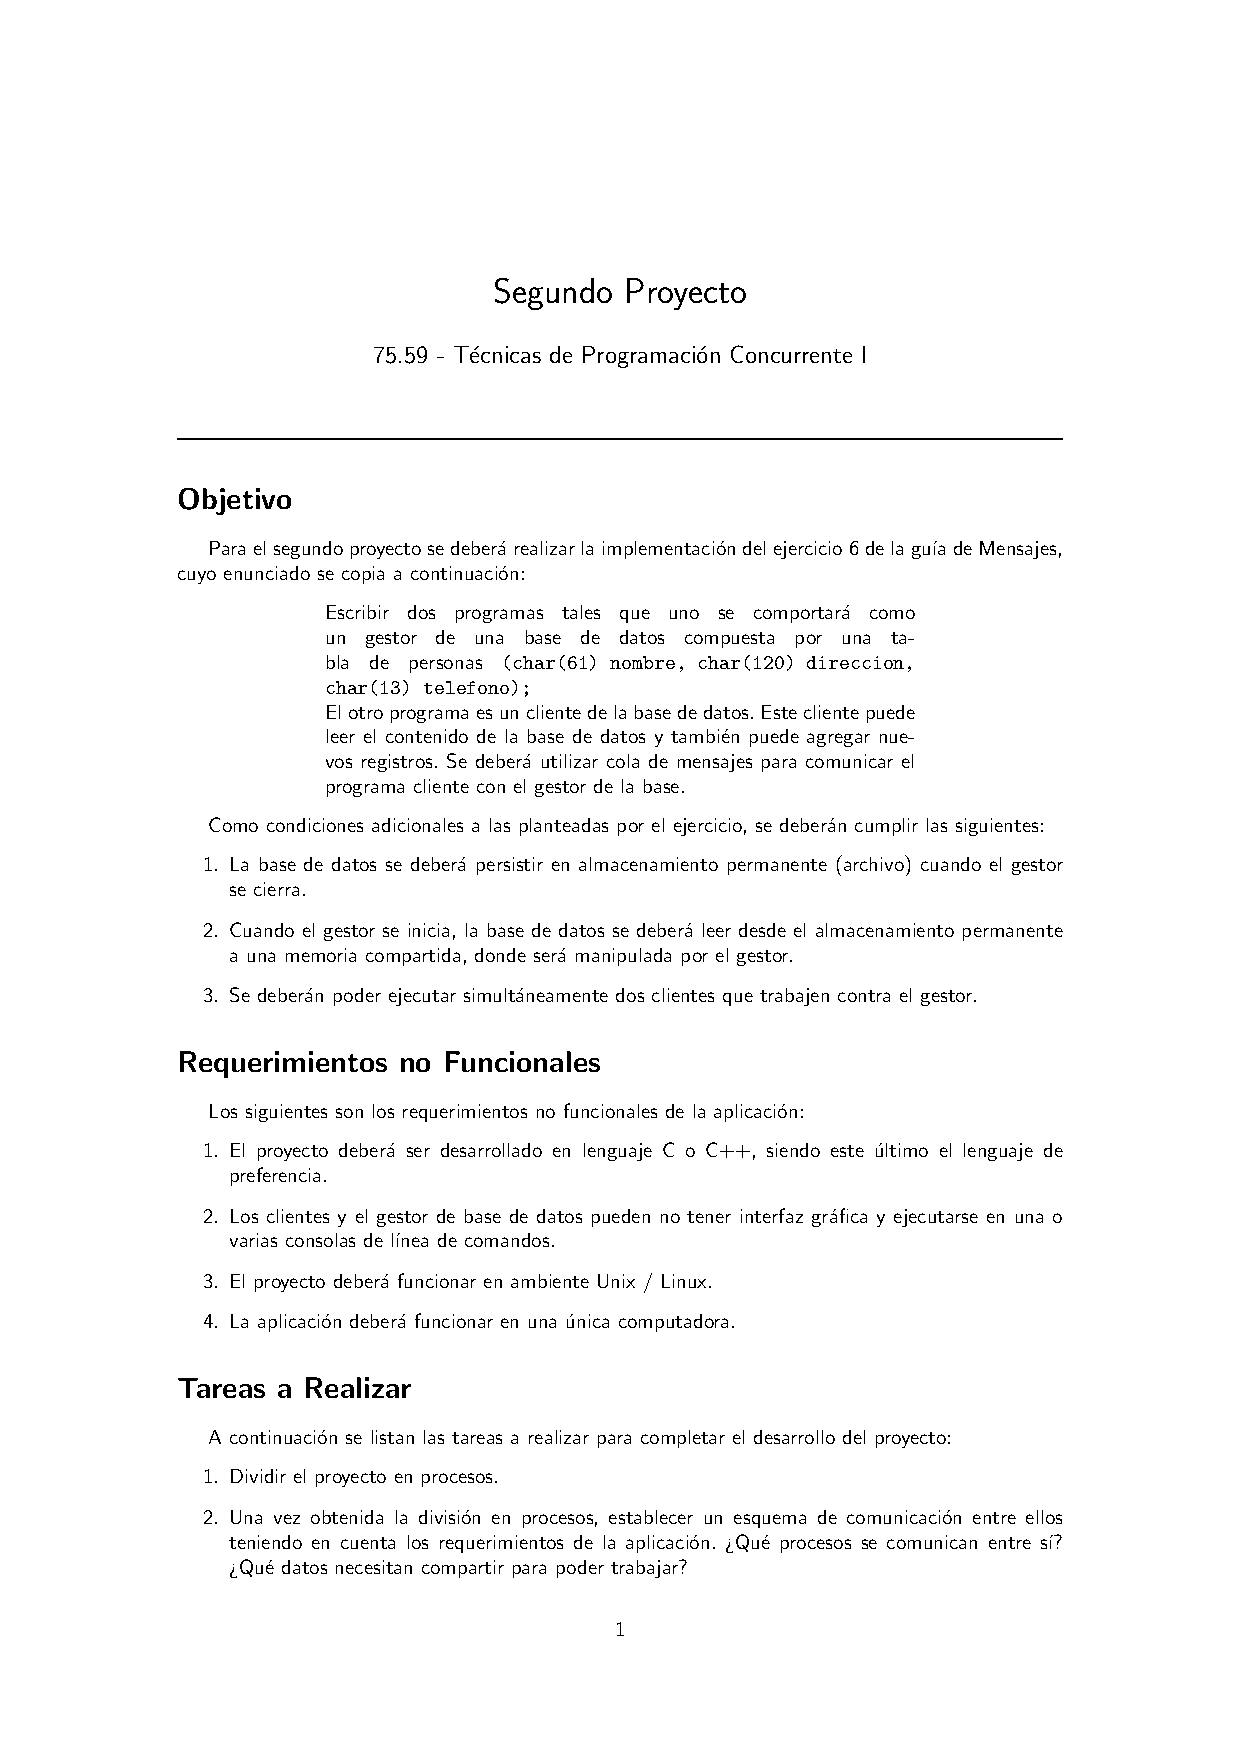
\includegraphics[trim = 25mm 30mm 10mm 35mm, clip,height=0.93\textheight,width=1.04\textwidth]{SegundoProyecto.pdf}
\includegraphics[trim = 25mm 20mm 10mm 30mm, clip,height=0.95\textheight,width=1.04\textwidth,page={2}]{SegundoProyecto.pdf}
\end{center}

\newpage


\section{Requerimientos Funcionales}

El sistema desarrollado permite realizar el alta, baja y modificaci\'on de los datos de una persona sobre la base de datos.
El mismo cuenta de dos aplicaciones diferentes, una aplicaci\'on cliente y una aplicaci\'on gestor.


\section{Hip\'otesis}
\begin{itemize}
 \item Se utiliz\'o como clave primaria de la base de datos el campo Nombre de cada registro. Es por este motivo, que se supone que si dos 
personas se llaman de igual forma, son la misma persona.

\end{itemize}


\section{Consideraciones de Dise\~no}

\begin{itemize}
\item Los campos permiten el ingreso de cadenas separadas por espacios, de forma tal de considerar los nombres compuestos, el ingreso de apellido y 
nombre de las personas, entre otras cosas.
\item Para el acceso a la memoria compartida se utiliz\'o un sem\'aforo de forma tal de lograr un sincronismo en el mismo. Este sem\'aforo es \'unico 
para la base de datos en su totalidad.
\item La persistencia de la base de datos {\bf TODO}
\item Al modificar una persona desde la aplicaci\'on cliente se le solicita al usuario que ingrese primero el nombre de la misma tal cual figura en la base de datos, 
y luego se le solicita que ingrese la nueva direcci\'on y tel\'efono. Siendo estos datos los almacenados a partir de dicho momento 
en la base de datos para la persona en cuesti\'on. Es decir, al modificar un registro de una persona se deben modificar los campos direcci\'on y tel\'efono de 
la misma. En caso de no querer modificar alguno, debe reingresarse la informaci\'on ya existente para dicho campo.

\end{itemize}

\section{Herramientas de concurrencia utilizadas}

Cola de mensajes \\
Memoria compartida \\
Sem\'aforo \\
LockFiles \\
Se\~nales \\

\section {Comunicaci\'on entre procesos}

Para realizar la comunicaci\'on entre los procesos gestor y cliente se utiliz\'o una \textit{Cola de Mensajes} dado que la misma permite comunicarlos 
aunque los mismos no posean relaci\'on entre ellos, como por ejemplo, en este caso, siendo dos aplicaciones diferentes. La ventaja que posee la 
cola de mensajes es que la misma permite enviar estructuras de datos completas a trav\'es de ella; en lugar de bytes como en los fifos.
Esto produce que no sea necesario sincronizar la escritura en la misma por mas que un proceso escriba en ella dado que no puede suspenderse la escritura 
de dicha estructura antes de finalizar, es decir, no puede darse el caso de que por cambiar el ipc el uso de cpu a otro proceso escriba uno la mitad de su estructura 
en la cola y el otro comience desde alli.
A su ves, la utilizaci\'on de colas de mensajes simplifica el protocolo de comunicaci\'on entre los procesos dado que es posible utilizar los campos de la estructura 
como por ejemplo, el dato long obligatorio para identificar a que proceso pertenece cada uno de los mensajes.

La estructura utilizada para transmitir los mensajes a trav\'es de la cola es la siguiente:

\begin{lstlisting}[language=C]
 typedef struct {
	long mtype;
	pid_t id;
	T_PETICION tipo;
	Registro registro;
	char respuesta[256];
} mensaje;
\end{lstlisting}

A continuaci\'on se presenta una descripci\'on de el significado y la utilizaci\'on de cada uno de los campos que conforman dicha estructura.
\begin{itemize}
 \item mtype:
\item id: es el n\'umero de proceso de quien env\'ia el mensaje.
\item tipo: es un enumerado que representa de que tipo de petici\'on proviene el mensaje en cuesti\'on. 
Los valores posibles para este campo son los siguientes: ``AGREGAR, ELIMINAR, CONSULTAR, MODIFICAR''
\item registro: es una estructura que contiene las cadenas de caracteres con los datos de la persona que se desea agregar, modificar, eliminar o sobre la que 
se desea consultar.
\item respuesta: es una cadena de caracteres que se utiliza para enviar mensajes de error o \'exito desde el gestor hacia los clientes, informandoles a 
trav\'es de estos el resultado de la operaci\'on realizada.
\end{itemize}


\subsection{Protocolo utilizado}

En cuanto al protocolo de comunicaci\'on utilizado, el mismo se desprende de observar la estructura anterior. 



\section{Casos de Uso}

\subsection{Cliente}

\begin{center}
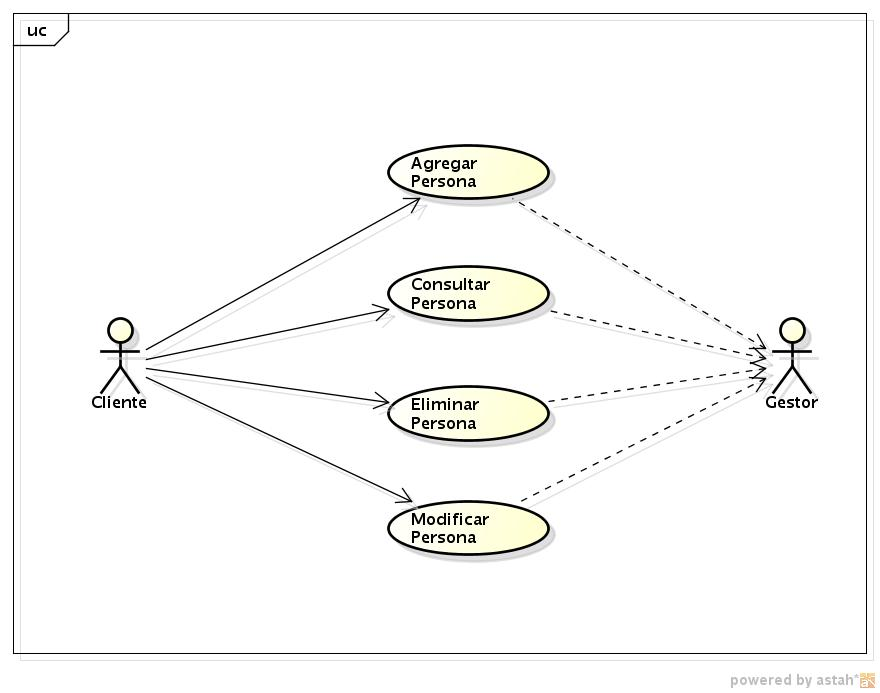
\includegraphics[scale=0.65]{CasosUsoCliente} 
\end{center}

\subsubsection{Especificaci\'on de los casos de uso del Cliente}

\subsection{Gestor}

%\begin{center}
%\includegraphics[scale=0.65]{CasosUsoGestor} 
%\end{center}

\subsubsection{Especificaci\'on de los casos de uso del Gestor}





\newpage

\section{Diagrama de clases}

\subsection{Diagrama de clases Cliente}

\subsection{Diagrama de clases Gestor}

\newpage
\section{Compilaci\'on}
Con el fin de facilitar la compilaci\'on de las aplicaciones se provee un archivo de {\bf Makefile}; el mismo se encuentra ubicado en 
el directorio en el cu\'al se encuentra el c\'odigo fuente. \\
El mismo se utiliza de la siguiente forma:
\begin{itemize}
 \item Ubicarse en el directorio en el cu\'al se encuentra el c\'odigo fuente de las aplicaciones. Para ello puede utilizarse el siguiente 
comando desde un ambiente Unix\/Linux:\\
\$~:cd Directorio\_del\_trabajo\_practico
\item Ejecutar el siguiente comando: \\
\$~:make all
\subitem * Se debe contar con el comando {\bf make} instalado en el sistema para poder compilar la aplicaci\'on de este modo.
\item Una vez finalizada la compilaci\'on del paso anterior, se observar\'an, en dicho directorio, dos archivos ejecutables: \textit{cliente} y \textit{gestor}. 
Estos archivos representan respectivamente a las aplicaciones cliente( para ejecutar los clientes debe utilizarse {\bf ./cliente}) y gestor({\bf ./gestor}). 
\end{itemize}


\section{Modo de Uso}
Para utilizar la aplicaci\'on {\bf gestor} debe considerarse que la misma finaliza al presionar la tecla \textit{'s'} en la consola en la cu\'al esta corriendo; 
esto es informado en la misma mediante un mensaje. \\ \\
Para utilizar la aplicaci\'on {\bf cliente} se debe respetar la interfaz por consola que la misma presenta. \\
Al momento de querer \underline{modificar} una persona desde la aplicaci\'on se debe ingresar el nombre de la misma tal cu\'al figura en la base de datos, dado que el mismo 
es la clave primaria.


\newpage


\section{Conclusiones}



\end{document}

